\pagebreak
\subsection{Implementing Jacobi and Gauss-Seidel Smoothers}
%Implement the Jacobi and Gauss-Seidel smoothers. Plot the $L_2$ residual norm convergence history of the Jacobi smoother for $p = 3$, using under-relaxation factors of $\omega = 0.3, 0.6, 1.0$. Do this for the first few hundred iterations and discuss the effect of under relaxation. Next, make a separate plot of the $L_2$ residual norm convergence history of Gauss-Seidel using $\omega = 0.5, 1, 1.5$. Start from zero interior-node initial conditions for all of your runs. Discuss how the two histories compare and the effects of under-relaxation.}

In this task, I will implement both a Jacobi iterative smoother and a Gauss-Seidel smoother. Taking an iterative solution approach allows for easier implementation, but as a result will display a slower convergence. This convergence history will be highlighted here.

\subsubsection{Jacobi Iteration Smoother}
In order to implement the Jacobi Iteration Smoother I will use the expression for the next iteration state approximation shown below as,

\begin{equation}
    u_{i,j}^{n+1} = \frac{1}{4}\left(u_{i-1,j}^n + u_{i+1,j}^n + u_{i,j-1}^n + u_{i,j-1}^n + \Delta h^2f_i\right)
    \label{eqn:jacboi}
\end{equation}\myequations{Jacobi Iteration Update Expression}

Using Equation \ref{eqn:jacboi} above, and implementing into Python code shown in Appendix \ref{alg:jacobi}, I can use this to approximate the next iteration state values and iterate several times until the approximation matches that of the analytical. Choosing the iteration values I choose to pick a high value of iterations until the approximated solution matched that of Figure \ref{fig:solution}. Then from here I conducted an $L_2$ residual norm and its convergence shown below.

\begin{figure}[h]
    \centering
    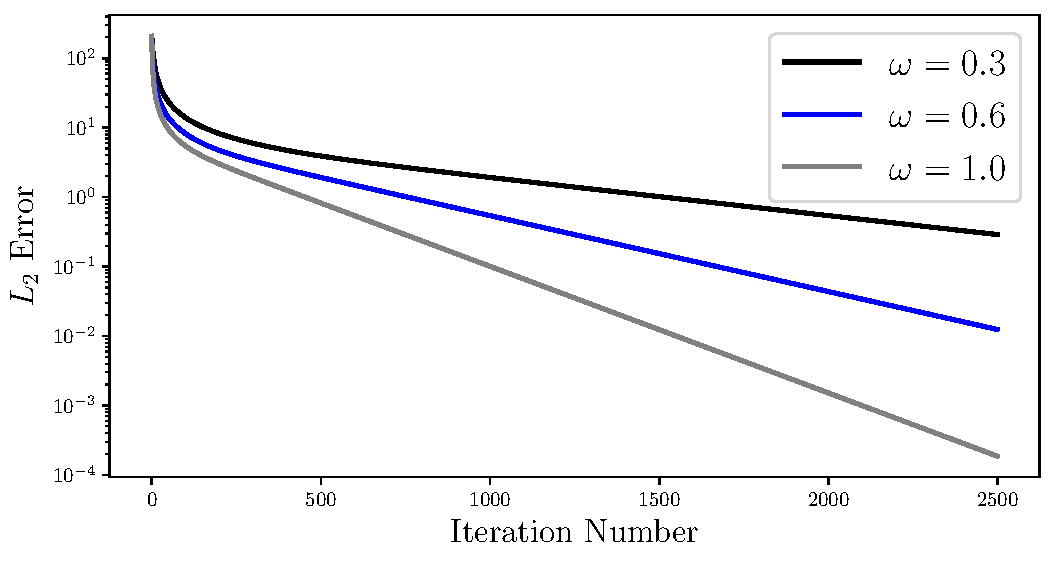
\includegraphics[width = 0.9\linewidth]{tasks/figs/jacobi_l2.pdf}
    \caption[Jacboi Smoother Iteration]{$L_2$ residual norm convergence history for varying $\omega$.}
    \label{fig:jacobi}
\end{figure}

As shown above in Figure \ref{fig:jacobi}, the over-relaxation factor plays a large role into how fast the solution converges. Further analysis on the $y$-$log$ plot shows that it appears as if the multiple of the over-relaxation factor of $\omega$ denotes what its $L_2$ error will be as $\omega = 0.6$ has an $L_2$ residual norm that is approximately twice the magnitude that of $\omega = 0.3$ residual norm.


\pagebreak
\subsubsection{Gauss-Seidel Smoother}
The Gauss-Seidel smoother is very similar in implementation to the Jacobi iteration smoother, however it differs in how the state updates. Gauss-Seidel will update half of the state first and then use the updated state to further smooth the approximated states in that given iteration. This method is called the ``\textit{checker-board}'' or black-red update. This essentially means that every other node/adjacent node will get updated and then use these updated nodes to make a better approximation. Implementing this in Python can be shown in Appendix \ref{alg:gauss}, but with the $L_2$ residual norm error shown below for differing values of over-relaxation.

\begin{figure}[h]
    \centering
    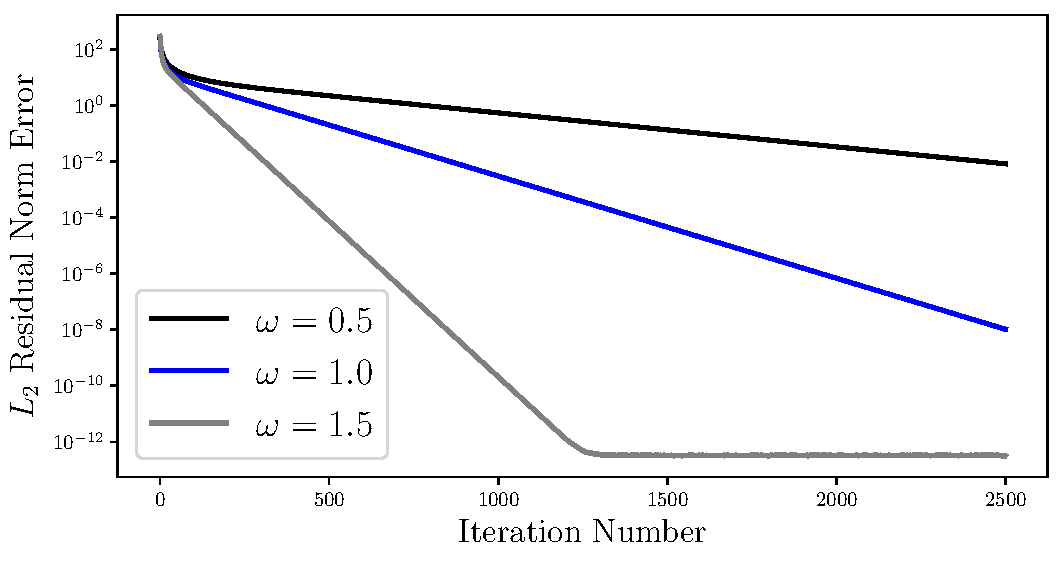
\includegraphics[width = 0.9\linewidth]{tasks/figs/gauss_l2.pdf}
    \caption[Gauss-Seidel Smoother]{$L_2$ residual norm convergence history for varying $\omega$.}
    \label{fig:gauss}
\end{figure}

Shown above in Figure \ref{fig:gauss}, is the $L_2$ residual norm error through its iteration values. This shows again the the over-relaxation value does converge faster with a higher value. However, this may be an artifact of machine precision but it does appear that $\omega = 1.5$ will converge to a given solution whereas $\omega = 0.5$ or $\omega = 1.0$ may be able to converge to a more precise solution but would take longer to do so.

\bigskip
\begin{fminipage}{0.9\linewidth}
    \textbf{Across both the Jacobi iteration smoother and the Gauss-Seidel smoother, the rates at which they converge depend on the over-relaxation value. Having a higher over-relaxation value will allow the iterative solver to coverge faster. However, notable is that the Gauss-Seidel smoother can have a over-relaxation value greater than 1 or $\bf \omega > 1$ and still converge. When Jacobi iteration smoother has an over-relaxation value greater than 1 it will diverge from the analytical solution whereas Gauss-Seidel continues to converge. Running Jacobi iteration with $\bf \omega = 1.1$ gave that the final value was $\bf \mathcal{O}(10^{140})$ which is in agreement that an over-relaxation value greater than 1 will diverge.}
\end{fminipage}